% Created by tikzDevice version 0.10.1 on 2017-11-22 12:37:07
% !TEX encoding = UTF-8 Unicode
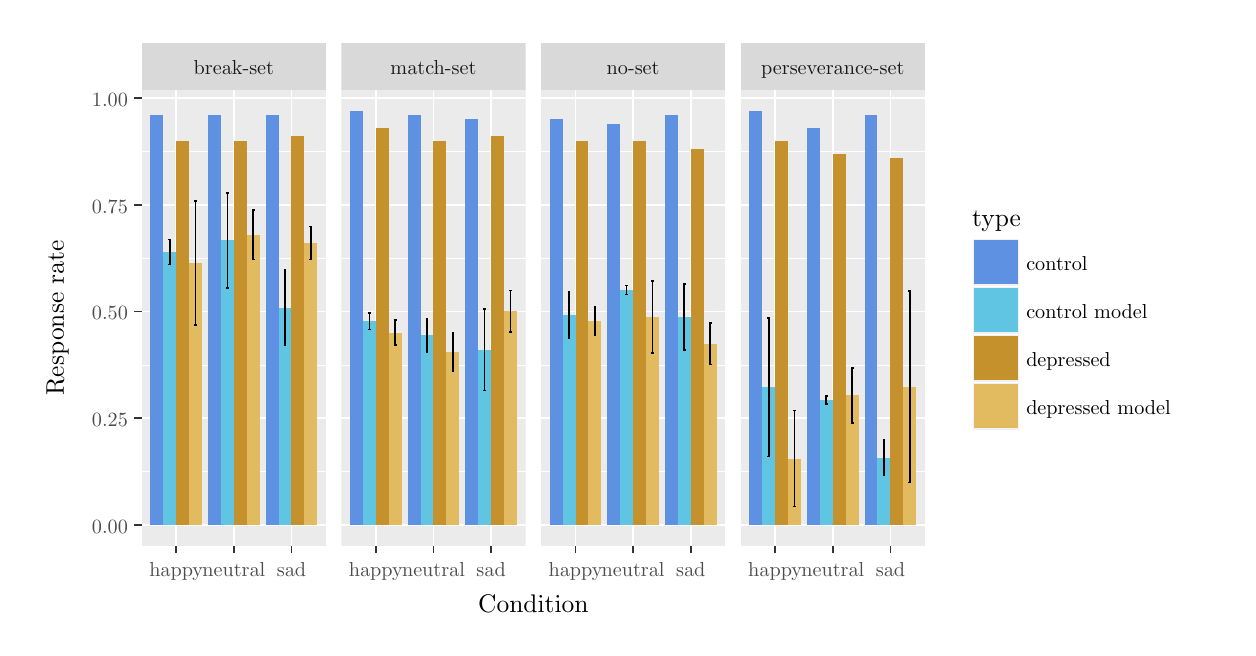
\begin{tikzpicture}[x=1pt,y=1pt]
\definecolor{fillColor}{RGB}{255,255,255}
\path[use as bounding box,fill=fillColor,fill opacity=0.00] (0,0) rectangle (433.62,216.81);
\begin{scope}
\path[clip] (  0.00,  0.00) rectangle (433.62,216.81);
\definecolor{drawColor}{RGB}{255,255,255}
\definecolor{fillColor}{RGB}{255,255,255}

\path[draw=drawColor,line width= 0.6pt,line join=round,line cap=round,fill=fillColor] (  0.00,  0.00) rectangle (433.62,216.81);
\end{scope}
\begin{scope}
\path[clip] ( 41.17, 29.59) rectangle (107.82,194.25);
\definecolor{fillColor}{gray}{0.92}

\path[fill=fillColor] ( 41.17, 29.59) rectangle (107.82,194.25);
\definecolor{drawColor}{RGB}{255,255,255}

\path[draw=drawColor,line width= 0.3pt,line join=round] ( 41.17, 56.36) --
	(107.82, 56.36);

\path[draw=drawColor,line width= 0.3pt,line join=round] ( 41.17, 94.94) --
	(107.82, 94.94);

\path[draw=drawColor,line width= 0.3pt,line join=round] ( 41.17,133.52) --
	(107.82,133.52);

\path[draw=drawColor,line width= 0.3pt,line join=round] ( 41.17,172.10) --
	(107.82,172.10);

\path[draw=drawColor,line width= 0.6pt,line join=round] ( 41.17, 37.07) --
	(107.82, 37.07);

\path[draw=drawColor,line width= 0.6pt,line join=round] ( 41.17, 75.65) --
	(107.82, 75.65);

\path[draw=drawColor,line width= 0.6pt,line join=round] ( 41.17,114.23) --
	(107.82,114.23);

\path[draw=drawColor,line width= 0.6pt,line join=round] ( 41.17,152.81) --
	(107.82,152.81);

\path[draw=drawColor,line width= 0.6pt,line join=round] ( 41.17,191.39) --
	(107.82,191.39);

\path[draw=drawColor,line width= 0.6pt,line join=round] ( 53.67, 29.59) --
	( 53.67,194.25);

\path[draw=drawColor,line width= 0.6pt,line join=round] ( 74.50, 29.59) --
	( 74.50,194.25);

\path[draw=drawColor,line width= 0.6pt,line join=round] ( 95.32, 29.59) --
	( 95.32,194.25);
\definecolor{fillColor}{RGB}{226,186,95}

\path[fill=fillColor] ( 58.36, 37.07) rectangle ( 63.04,131.74);
\definecolor{fillColor}{RGB}{196,145,45}

\path[fill=fillColor] ( 53.67, 37.07) rectangle ( 58.36,175.96);
\definecolor{fillColor}{RGB}{95,197,226}

\path[fill=fillColor] ( 48.98, 37.07) rectangle ( 53.67,135.75);
\definecolor{fillColor}{RGB}{95,145,226}

\path[fill=fillColor] ( 44.30, 37.07) rectangle ( 48.98,185.22);
\definecolor{fillColor}{RGB}{226,186,95}

\path[fill=fillColor] ( 79.18, 37.07) rectangle ( 83.87,141.92);
\definecolor{fillColor}{RGB}{196,145,45}

\path[fill=fillColor] ( 74.50, 37.07) rectangle ( 79.18,175.96);
\definecolor{fillColor}{RGB}{95,197,226}

\path[fill=fillColor] ( 69.81, 37.07) rectangle ( 74.50,139.95);
\definecolor{fillColor}{RGB}{95,145,226}

\path[fill=fillColor] ( 65.12, 37.07) rectangle ( 69.81,185.22);
\definecolor{fillColor}{RGB}{226,186,95}

\path[fill=fillColor] (100.01, 37.07) rectangle (104.69,138.99);
\definecolor{fillColor}{RGB}{196,145,45}

\path[fill=fillColor] ( 95.32, 37.07) rectangle (100.01,177.51);
\definecolor{fillColor}{RGB}{95,197,226}

\path[fill=fillColor] ( 90.64, 37.07) rectangle ( 95.32,115.66);
\definecolor{fillColor}{RGB}{95,145,226}

\path[fill=fillColor] ( 85.95, 37.07) rectangle ( 90.64,185.22);
\definecolor{drawColor}{RGB}{0,0,0}

\path[draw=drawColor,line width= 0.6pt,line join=round] ( 60.18,154.23) --
	( 61.22,154.23);

\path[draw=drawColor,line width= 0.6pt,line join=round] ( 60.70,154.23) --
	( 60.70,109.25);

\path[draw=drawColor,line width= 0.6pt,line join=round] ( 60.18,109.25) --
	( 61.22,109.25);

\path[draw=drawColor,line width= 0.6pt,line join=round] ( 50.81,140.24) --
	( 51.85,140.24);

\path[draw=drawColor,line width= 0.6pt,line join=round] ( 51.33,140.24) --
	( 51.33,131.25);

\path[draw=drawColor,line width= 0.6pt,line join=round] ( 50.81,131.25) --
	( 51.85,131.25);

\path[draw=drawColor,line width= 0.6pt,line join=round] ( 81.00,150.83) --
	( 82.05,150.83);

\path[draw=drawColor,line width= 0.6pt,line join=round] ( 81.52,150.83) --
	( 81.52,133.02);

\path[draw=drawColor,line width= 0.6pt,line join=round] ( 81.00,133.02) --
	( 82.05,133.02);

\path[draw=drawColor,line width= 0.6pt,line join=round] ( 71.63,157.10) --
	( 72.67,157.10);

\path[draw=drawColor,line width= 0.6pt,line join=round] ( 72.15,157.10) --
	( 72.15,122.81);

\path[draw=drawColor,line width= 0.6pt,line join=round] ( 71.63,122.81) --
	( 72.67,122.81);

\path[draw=drawColor,line width= 0.6pt,line join=round] (101.83,144.96) --
	(102.87,144.96);

\path[draw=drawColor,line width= 0.6pt,line join=round] (102.35,144.96) --
	(102.35,133.03);

\path[draw=drawColor,line width= 0.6pt,line join=round] (101.83,133.03) --
	(102.87,133.03);

\path[draw=drawColor,line width= 0.6pt,line join=round] ( 92.46,129.33) --
	( 93.50,129.33);

\path[draw=drawColor,line width= 0.6pt,line join=round] ( 92.98,129.33) --
	( 92.98,101.99);

\path[draw=drawColor,line width= 0.6pt,line join=round] ( 92.46,101.99) --
	( 93.50,101.99);
\end{scope}
\begin{scope}
\path[clip] (113.32, 29.59) rectangle (179.96,194.25);
\definecolor{fillColor}{gray}{0.92}

\path[fill=fillColor] (113.32, 29.59) rectangle (179.96,194.25);
\definecolor{drawColor}{RGB}{255,255,255}

\path[draw=drawColor,line width= 0.3pt,line join=round] (113.32, 56.36) --
	(179.96, 56.36);

\path[draw=drawColor,line width= 0.3pt,line join=round] (113.32, 94.94) --
	(179.96, 94.94);

\path[draw=drawColor,line width= 0.3pt,line join=round] (113.32,133.52) --
	(179.96,133.52);

\path[draw=drawColor,line width= 0.3pt,line join=round] (113.32,172.10) --
	(179.96,172.10);

\path[draw=drawColor,line width= 0.6pt,line join=round] (113.32, 37.07) --
	(179.96, 37.07);

\path[draw=drawColor,line width= 0.6pt,line join=round] (113.32, 75.65) --
	(179.96, 75.65);

\path[draw=drawColor,line width= 0.6pt,line join=round] (113.32,114.23) --
	(179.96,114.23);

\path[draw=drawColor,line width= 0.6pt,line join=round] (113.32,152.81) --
	(179.96,152.81);

\path[draw=drawColor,line width= 0.6pt,line join=round] (113.32,191.39) --
	(179.96,191.39);

\path[draw=drawColor,line width= 0.6pt,line join=round] (125.81, 29.59) --
	(125.81,194.25);

\path[draw=drawColor,line width= 0.6pt,line join=round] (146.64, 29.59) --
	(146.64,194.25);

\path[draw=drawColor,line width= 0.6pt,line join=round] (167.47, 29.59) --
	(167.47,194.25);
\definecolor{fillColor}{RGB}{226,186,95}

\path[fill=fillColor] (130.50, 37.07) rectangle (135.19,106.63);
\definecolor{fillColor}{RGB}{196,145,45}

\path[fill=fillColor] (125.81, 37.07) rectangle (130.50,180.59);
\definecolor{fillColor}{RGB}{95,197,226}

\path[fill=fillColor] (121.13, 37.07) rectangle (125.81,110.78);
\definecolor{fillColor}{RGB}{95,145,226}

\path[fill=fillColor] (116.44, 37.07) rectangle (121.13,186.76);
\definecolor{fillColor}{RGB}{226,186,95}

\path[fill=fillColor] (151.33, 37.07) rectangle (156.01, 99.66);
\definecolor{fillColor}{RGB}{196,145,45}

\path[fill=fillColor] (146.64, 37.07) rectangle (151.33,175.96);
\definecolor{fillColor}{RGB}{95,197,226}

\path[fill=fillColor] (141.95, 37.07) rectangle (146.64,105.74);
\definecolor{fillColor}{RGB}{95,145,226}

\path[fill=fillColor] (137.27, 37.07) rectangle (141.95,185.22);
\definecolor{fillColor}{RGB}{226,186,95}

\path[fill=fillColor] (172.15, 37.07) rectangle (176.84,114.36);
\definecolor{fillColor}{RGB}{196,145,45}

\path[fill=fillColor] (167.47, 37.07) rectangle (172.15,177.51);
\definecolor{fillColor}{RGB}{95,197,226}

\path[fill=fillColor] (162.78, 37.07) rectangle (167.47,100.46);
\definecolor{fillColor}{RGB}{95,145,226}

\path[fill=fillColor] (158.10, 37.07) rectangle (162.78,183.68);
\definecolor{drawColor}{RGB}{0,0,0}

\path[draw=drawColor,line width= 0.6pt,line join=round] (132.32,111.06) --
	(133.36,111.06);

\path[draw=drawColor,line width= 0.6pt,line join=round] (132.84,111.06) --
	(132.84,102.21);

\path[draw=drawColor,line width= 0.6pt,line join=round] (132.32,102.21) --
	(133.36,102.21);

\path[draw=drawColor,line width= 0.6pt,line join=round] (122.95,113.81) --
	(123.99,113.81);

\path[draw=drawColor,line width= 0.6pt,line join=round] (123.47,113.81) --
	(123.47,107.75);

\path[draw=drawColor,line width= 0.6pt,line join=round] (122.95,107.75) --
	(123.99,107.75);

\path[draw=drawColor,line width= 0.6pt,line join=round] (153.15,106.68) --
	(154.19,106.68);

\path[draw=drawColor,line width= 0.6pt,line join=round] (153.67,106.68) --
	(153.67, 92.64);

\path[draw=drawColor,line width= 0.6pt,line join=round] (153.15, 92.64) --
	(154.19, 92.64);

\path[draw=drawColor,line width= 0.6pt,line join=round] (143.78,111.76) --
	(144.82,111.76);

\path[draw=drawColor,line width= 0.6pt,line join=round] (144.30,111.76) --
	(144.30, 99.72);

\path[draw=drawColor,line width= 0.6pt,line join=round] (143.78, 99.72) --
	(144.82, 99.72);

\path[draw=drawColor,line width= 0.6pt,line join=round] (173.98,121.89) --
	(175.02,121.89);

\path[draw=drawColor,line width= 0.6pt,line join=round] (174.50,121.89) --
	(174.50,106.82);

\path[draw=drawColor,line width= 0.6pt,line join=round] (173.98,106.82) --
	(175.02,106.82);

\path[draw=drawColor,line width= 0.6pt,line join=round] (164.60,115.27) --
	(165.64,115.27);

\path[draw=drawColor,line width= 0.6pt,line join=round] (165.12,115.27) --
	(165.12, 85.65);

\path[draw=drawColor,line width= 0.6pt,line join=round] (164.60, 85.65) --
	(165.64, 85.65);
\end{scope}
\begin{scope}
\path[clip] (185.46, 29.59) rectangle (252.11,194.25);
\definecolor{fillColor}{gray}{0.92}

\path[fill=fillColor] (185.46, 29.59) rectangle (252.11,194.25);
\definecolor{drawColor}{RGB}{255,255,255}

\path[draw=drawColor,line width= 0.3pt,line join=round] (185.46, 56.36) --
	(252.11, 56.36);

\path[draw=drawColor,line width= 0.3pt,line join=round] (185.46, 94.94) --
	(252.11, 94.94);

\path[draw=drawColor,line width= 0.3pt,line join=round] (185.46,133.52) --
	(252.11,133.52);

\path[draw=drawColor,line width= 0.3pt,line join=round] (185.46,172.10) --
	(252.11,172.10);

\path[draw=drawColor,line width= 0.6pt,line join=round] (185.46, 37.07) --
	(252.11, 37.07);

\path[draw=drawColor,line width= 0.6pt,line join=round] (185.46, 75.65) --
	(252.11, 75.65);

\path[draw=drawColor,line width= 0.6pt,line join=round] (185.46,114.23) --
	(252.11,114.23);

\path[draw=drawColor,line width= 0.6pt,line join=round] (185.46,152.81) --
	(252.11,152.81);

\path[draw=drawColor,line width= 0.6pt,line join=round] (185.46,191.39) --
	(252.11,191.39);

\path[draw=drawColor,line width= 0.6pt,line join=round] (197.96, 29.59) --
	(197.96,194.25);

\path[draw=drawColor,line width= 0.6pt,line join=round] (218.79, 29.59) --
	(218.79,194.25);

\path[draw=drawColor,line width= 0.6pt,line join=round] (239.61, 29.59) --
	(239.61,194.25);
\definecolor{fillColor}{RGB}{226,186,95}

\path[fill=fillColor] (202.64, 37.07) rectangle (207.33,110.70);
\definecolor{fillColor}{RGB}{196,145,45}

\path[fill=fillColor] (197.96, 37.07) rectangle (202.64,175.96);
\definecolor{fillColor}{RGB}{95,197,226}

\path[fill=fillColor] (193.27, 37.07) rectangle (197.96,112.95);
\definecolor{fillColor}{RGB}{95,145,226}

\path[fill=fillColor] (188.59, 37.07) rectangle (193.27,183.68);
\definecolor{fillColor}{RGB}{226,186,95}

\path[fill=fillColor] (223.47, 37.07) rectangle (228.16,112.36);
\definecolor{fillColor}{RGB}{196,145,45}

\path[fill=fillColor] (218.79, 37.07) rectangle (223.47,175.96);
\definecolor{fillColor}{RGB}{95,197,226}

\path[fill=fillColor] (214.10, 37.07) rectangle (218.79,122.03);
\definecolor{fillColor}{RGB}{95,145,226}

\path[fill=fillColor] (209.41, 37.07) rectangle (214.10,182.14);
\definecolor{fillColor}{RGB}{226,186,95}

\path[fill=fillColor] (244.30, 37.07) rectangle (248.98,102.62);
\definecolor{fillColor}{RGB}{196,145,45}

\path[fill=fillColor] (239.61, 37.07) rectangle (244.30,172.88);
\definecolor{fillColor}{RGB}{95,197,226}

\path[fill=fillColor] (234.93, 37.07) rectangle (239.61,112.29);
\definecolor{fillColor}{RGB}{95,145,226}

\path[fill=fillColor] (230.24, 37.07) rectangle (234.93,185.22);
\definecolor{drawColor}{RGB}{0,0,0}

\path[draw=drawColor,line width= 0.6pt,line join=round] (204.47,115.88) --
	(205.51,115.88);

\path[draw=drawColor,line width= 0.6pt,line join=round] (204.99,115.88) --
	(204.99,105.52);

\path[draw=drawColor,line width= 0.6pt,line join=round] (204.47,105.52) --
	(205.51,105.52);

\path[draw=drawColor,line width= 0.6pt,line join=round] (195.10,121.43) --
	(196.14,121.43);

\path[draw=drawColor,line width= 0.6pt,line join=round] (195.62,121.43) --
	(195.62,104.48);

\path[draw=drawColor,line width= 0.6pt,line join=round] (195.10,104.48) --
	(196.14,104.48);

\path[draw=drawColor,line width= 0.6pt,line join=round] (225.29,125.38) --
	(226.34,125.38);

\path[draw=drawColor,line width= 0.6pt,line join=round] (225.81,125.38) --
	(225.81, 99.34);

\path[draw=drawColor,line width= 0.6pt,line join=round] (225.29, 99.34) --
	(226.34, 99.34);

\path[draw=drawColor,line width= 0.6pt,line join=round] (215.92,123.70) --
	(216.96,123.70);

\path[draw=drawColor,line width= 0.6pt,line join=round] (216.44,123.70) --
	(216.44,120.36);

\path[draw=drawColor,line width= 0.6pt,line join=round] (215.92,120.36) --
	(216.96,120.36);

\path[draw=drawColor,line width= 0.6pt,line join=round] (246.12,110.12) --
	(247.16,110.12);

\path[draw=drawColor,line width= 0.6pt,line join=round] (246.64,110.12) --
	(246.64, 95.11);

\path[draw=drawColor,line width= 0.6pt,line join=round] (246.12, 95.11) --
	(247.16, 95.11);

\path[draw=drawColor,line width= 0.6pt,line join=round] (236.75,124.23) --
	(237.79,124.23);

\path[draw=drawColor,line width= 0.6pt,line join=round] (237.27,124.23) --
	(237.27,100.36);

\path[draw=drawColor,line width= 0.6pt,line join=round] (236.75,100.36) --
	(237.79,100.36);
\end{scope}
\begin{scope}
\path[clip] (257.61, 29.59) rectangle (324.25,194.25);
\definecolor{fillColor}{gray}{0.92}

\path[fill=fillColor] (257.61, 29.59) rectangle (324.25,194.25);
\definecolor{drawColor}{RGB}{255,255,255}

\path[draw=drawColor,line width= 0.3pt,line join=round] (257.61, 56.36) --
	(324.25, 56.36);

\path[draw=drawColor,line width= 0.3pt,line join=round] (257.61, 94.94) --
	(324.25, 94.94);

\path[draw=drawColor,line width= 0.3pt,line join=round] (257.61,133.52) --
	(324.25,133.52);

\path[draw=drawColor,line width= 0.3pt,line join=round] (257.61,172.10) --
	(324.25,172.10);

\path[draw=drawColor,line width= 0.6pt,line join=round] (257.61, 37.07) --
	(324.25, 37.07);

\path[draw=drawColor,line width= 0.6pt,line join=round] (257.61, 75.65) --
	(324.25, 75.65);

\path[draw=drawColor,line width= 0.6pt,line join=round] (257.61,114.23) --
	(324.25,114.23);

\path[draw=drawColor,line width= 0.6pt,line join=round] (257.61,152.81) --
	(324.25,152.81);

\path[draw=drawColor,line width= 0.6pt,line join=round] (257.61,191.39) --
	(324.25,191.39);

\path[draw=drawColor,line width= 0.6pt,line join=round] (270.10, 29.59) --
	(270.10,194.25);

\path[draw=drawColor,line width= 0.6pt,line join=round] (290.93, 29.59) --
	(290.93,194.25);

\path[draw=drawColor,line width= 0.6pt,line join=round] (311.76, 29.59) --
	(311.76,194.25);
\definecolor{fillColor}{RGB}{226,186,95}

\path[fill=fillColor] (274.79, 37.07) rectangle (279.48, 61.12);
\definecolor{fillColor}{RGB}{196,145,45}

\path[fill=fillColor] (270.10, 37.07) rectangle (274.79,175.96);
\definecolor{fillColor}{RGB}{95,197,226}

\path[fill=fillColor] (265.42, 37.07) rectangle (270.10, 86.84);
\definecolor{fillColor}{RGB}{95,145,226}

\path[fill=fillColor] (260.73, 37.07) rectangle (265.42,186.76);
\definecolor{fillColor}{RGB}{226,186,95}

\path[fill=fillColor] (295.62, 37.07) rectangle (300.30, 83.92);
\definecolor{fillColor}{RGB}{196,145,45}

\path[fill=fillColor] (290.93, 37.07) rectangle (295.62,171.33);
\definecolor{fillColor}{RGB}{95,197,226}

\path[fill=fillColor] (286.24, 37.07) rectangle (290.93, 82.27);
\definecolor{fillColor}{RGB}{95,145,226}

\path[fill=fillColor] (281.56, 37.07) rectangle (286.24,180.59);
\definecolor{fillColor}{RGB}{226,186,95}

\path[fill=fillColor] (316.44, 37.07) rectangle (321.13, 87.04);
\definecolor{fillColor}{RGB}{196,145,45}

\path[fill=fillColor] (311.76, 37.07) rectangle (316.44,169.79);
\definecolor{fillColor}{RGB}{95,197,226}

\path[fill=fillColor] (307.07, 37.07) rectangle (311.76, 61.49);
\definecolor{fillColor}{RGB}{95,145,226}

\path[fill=fillColor] (302.39, 37.07) rectangle (307.07,185.22);
\definecolor{drawColor}{RGB}{0,0,0}

\path[draw=drawColor,line width= 0.6pt,line join=round] (276.61, 78.48) --
	(277.65, 78.48);

\path[draw=drawColor,line width= 0.6pt,line join=round] (277.13, 78.48) --
	(277.13, 43.76);

\path[draw=drawColor,line width= 0.6pt,line join=round] (276.61, 43.76) --
	(277.65, 43.76);

\path[draw=drawColor,line width= 0.6pt,line join=round] (267.24,111.88) --
	(268.28,111.88);

\path[draw=drawColor,line width= 0.6pt,line join=round] (267.76,111.88) --
	(267.76, 61.80);

\path[draw=drawColor,line width= 0.6pt,line join=round] (267.24, 61.80) --
	(268.28, 61.80);

\path[draw=drawColor,line width= 0.6pt,line join=round] (297.44, 93.86) --
	(298.48, 93.86);

\path[draw=drawColor,line width= 0.6pt,line join=round] (297.96, 93.86) --
	(297.96, 73.98);

\path[draw=drawColor,line width= 0.6pt,line join=round] (297.44, 73.98) --
	(298.48, 73.98);

\path[draw=drawColor,line width= 0.6pt,line join=round] (288.07, 83.82) --
	(289.11, 83.82);

\path[draw=drawColor,line width= 0.6pt,line join=round] (288.59, 83.82) --
	(288.59, 80.71);

\path[draw=drawColor,line width= 0.6pt,line join=round] (288.07, 80.71) --
	(289.11, 80.71);

\path[draw=drawColor,line width= 0.6pt,line join=round] (318.27,121.64) --
	(319.31,121.64);

\path[draw=drawColor,line width= 0.6pt,line join=round] (318.79,121.64) --
	(318.79, 52.44);

\path[draw=drawColor,line width= 0.6pt,line join=round] (318.27, 52.44) --
	(319.31, 52.44);

\path[draw=drawColor,line width= 0.6pt,line join=round] (308.89, 67.79) --
	(309.93, 67.79);

\path[draw=drawColor,line width= 0.6pt,line join=round] (309.41, 67.79) --
	(309.41, 55.19);

\path[draw=drawColor,line width= 0.6pt,line join=round] (308.89, 55.19) --
	(309.93, 55.19);
\end{scope}
\begin{scope}
\path[clip] ( 41.17,194.25) rectangle (107.82,211.31);
\definecolor{fillColor}{gray}{0.85}

\path[fill=fillColor] ( 41.17,194.25) rectangle (107.82,211.31);
\definecolor{drawColor}{gray}{0.10}

\node[text=drawColor,anchor=base,inner sep=0pt, outer sep=0pt, scale=  0.73] at ( 74.50,199.75) {break-set};
\end{scope}
\begin{scope}
\path[clip] (113.32,194.25) rectangle (179.96,211.31);
\definecolor{fillColor}{gray}{0.85}

\path[fill=fillColor] (113.32,194.25) rectangle (179.96,211.31);
\definecolor{drawColor}{gray}{0.10}

\node[text=drawColor,anchor=base,inner sep=0pt, outer sep=0pt, scale=  0.73] at (146.64,199.75) {match-set};
\end{scope}
\begin{scope}
\path[clip] (185.46,194.25) rectangle (252.11,211.31);
\definecolor{fillColor}{gray}{0.85}

\path[fill=fillColor] (185.46,194.25) rectangle (252.11,211.31);
\definecolor{drawColor}{gray}{0.10}

\node[text=drawColor,anchor=base,inner sep=0pt, outer sep=0pt, scale=  0.73] at (218.79,199.75) {no-set};
\end{scope}
\begin{scope}
\path[clip] (257.61,194.25) rectangle (324.25,211.31);
\definecolor{fillColor}{gray}{0.85}

\path[fill=fillColor] (257.61,194.25) rectangle (324.25,211.31);
\definecolor{drawColor}{gray}{0.10}

\node[text=drawColor,anchor=base,inner sep=0pt, outer sep=0pt, scale=  0.73] at (290.93,199.75) {perseverance-set};
\end{scope}
\begin{scope}
\path[clip] (  0.00,  0.00) rectangle (433.62,216.81);
\definecolor{drawColor}{gray}{0.20}

\path[draw=drawColor,line width= 0.6pt,line join=round] ( 53.67, 26.84) --
	( 53.67, 29.59);

\path[draw=drawColor,line width= 0.6pt,line join=round] ( 74.50, 26.84) --
	( 74.50, 29.59);

\path[draw=drawColor,line width= 0.6pt,line join=round] ( 95.32, 26.84) --
	( 95.32, 29.59);
\end{scope}
\begin{scope}
\path[clip] (  0.00,  0.00) rectangle (433.62,216.81);
\definecolor{drawColor}{gray}{0.30}

\node[text=drawColor,anchor=base,inner sep=0pt, outer sep=0pt, scale=  0.73] at ( 53.67, 18.58) {happy};

\node[text=drawColor,anchor=base,inner sep=0pt, outer sep=0pt, scale=  0.73] at ( 74.50, 18.58) {neutral};

\node[text=drawColor,anchor=base,inner sep=0pt, outer sep=0pt, scale=  0.73] at ( 95.32, 18.58) {sad};
\end{scope}
\begin{scope}
\path[clip] (  0.00,  0.00) rectangle (433.62,216.81);
\definecolor{drawColor}{gray}{0.20}

\path[draw=drawColor,line width= 0.6pt,line join=round] (125.81, 26.84) --
	(125.81, 29.59);

\path[draw=drawColor,line width= 0.6pt,line join=round] (146.64, 26.84) --
	(146.64, 29.59);

\path[draw=drawColor,line width= 0.6pt,line join=round] (167.47, 26.84) --
	(167.47, 29.59);
\end{scope}
\begin{scope}
\path[clip] (  0.00,  0.00) rectangle (433.62,216.81);
\definecolor{drawColor}{gray}{0.30}

\node[text=drawColor,anchor=base,inner sep=0pt, outer sep=0pt, scale=  0.73] at (125.81, 18.58) {happy};

\node[text=drawColor,anchor=base,inner sep=0pt, outer sep=0pt, scale=  0.73] at (146.64, 18.58) {neutral};

\node[text=drawColor,anchor=base,inner sep=0pt, outer sep=0pt, scale=  0.73] at (167.47, 18.58) {sad};
\end{scope}
\begin{scope}
\path[clip] (  0.00,  0.00) rectangle (433.62,216.81);
\definecolor{drawColor}{gray}{0.20}

\path[draw=drawColor,line width= 0.6pt,line join=round] (197.96, 26.84) --
	(197.96, 29.59);

\path[draw=drawColor,line width= 0.6pt,line join=round] (218.79, 26.84) --
	(218.79, 29.59);

\path[draw=drawColor,line width= 0.6pt,line join=round] (239.61, 26.84) --
	(239.61, 29.59);
\end{scope}
\begin{scope}
\path[clip] (  0.00,  0.00) rectangle (433.62,216.81);
\definecolor{drawColor}{gray}{0.30}

\node[text=drawColor,anchor=base,inner sep=0pt, outer sep=0pt, scale=  0.73] at (197.96, 18.58) {happy};

\node[text=drawColor,anchor=base,inner sep=0pt, outer sep=0pt, scale=  0.73] at (218.79, 18.58) {neutral};

\node[text=drawColor,anchor=base,inner sep=0pt, outer sep=0pt, scale=  0.73] at (239.61, 18.58) {sad};
\end{scope}
\begin{scope}
\path[clip] (  0.00,  0.00) rectangle (433.62,216.81);
\definecolor{drawColor}{gray}{0.20}

\path[draw=drawColor,line width= 0.6pt,line join=round] (270.10, 26.84) --
	(270.10, 29.59);

\path[draw=drawColor,line width= 0.6pt,line join=round] (290.93, 26.84) --
	(290.93, 29.59);

\path[draw=drawColor,line width= 0.6pt,line join=round] (311.76, 26.84) --
	(311.76, 29.59);
\end{scope}
\begin{scope}
\path[clip] (  0.00,  0.00) rectangle (433.62,216.81);
\definecolor{drawColor}{gray}{0.30}

\node[text=drawColor,anchor=base,inner sep=0pt, outer sep=0pt, scale=  0.73] at (270.10, 18.58) {happy};

\node[text=drawColor,anchor=base,inner sep=0pt, outer sep=0pt, scale=  0.73] at (290.93, 18.58) {neutral};

\node[text=drawColor,anchor=base,inner sep=0pt, outer sep=0pt, scale=  0.73] at (311.76, 18.58) {sad};
\end{scope}
\begin{scope}
\path[clip] (  0.00,  0.00) rectangle (433.62,216.81);
\definecolor{drawColor}{gray}{0.30}

\node[text=drawColor,anchor=base east,inner sep=0pt, outer sep=0pt, scale=  0.73] at ( 36.22, 34.04) {0.00};

\node[text=drawColor,anchor=base east,inner sep=0pt, outer sep=0pt, scale=  0.73] at ( 36.22, 72.62) {0.25};

\node[text=drawColor,anchor=base east,inner sep=0pt, outer sep=0pt, scale=  0.73] at ( 36.22,111.20) {0.50};

\node[text=drawColor,anchor=base east,inner sep=0pt, outer sep=0pt, scale=  0.73] at ( 36.22,149.78) {0.75};

\node[text=drawColor,anchor=base east,inner sep=0pt, outer sep=0pt, scale=  0.73] at ( 36.22,188.36) {1.00};
\end{scope}
\begin{scope}
\path[clip] (  0.00,  0.00) rectangle (433.62,216.81);
\definecolor{drawColor}{gray}{0.20}

\path[draw=drawColor,line width= 0.6pt,line join=round] ( 38.42, 37.07) --
	( 41.17, 37.07);

\path[draw=drawColor,line width= 0.6pt,line join=round] ( 38.42, 75.65) --
	( 41.17, 75.65);

\path[draw=drawColor,line width= 0.6pt,line join=round] ( 38.42,114.23) --
	( 41.17,114.23);

\path[draw=drawColor,line width= 0.6pt,line join=round] ( 38.42,152.81) --
	( 41.17,152.81);

\path[draw=drawColor,line width= 0.6pt,line join=round] ( 38.42,191.39) --
	( 41.17,191.39);
\end{scope}
\begin{scope}
\path[clip] (  0.00,  0.00) rectangle (433.62,216.81);
\definecolor{drawColor}{RGB}{0,0,0}

\node[text=drawColor,anchor=base,inner sep=0pt, outer sep=0pt, scale=  0.92] at (182.71,  5.50) {Condition};
\end{scope}
\begin{scope}
\path[clip] (  0.00,  0.00) rectangle (433.62,216.81);
\definecolor{drawColor}{RGB}{0,0,0}

\node[text=drawColor,rotate= 90.00,anchor=base,inner sep=0pt, outer sep=0pt, scale=  0.92] at ( 13.08,111.92) {Response rate};
\end{scope}
\begin{scope}
\path[clip] (  0.00,  0.00) rectangle (433.62,216.81);
\definecolor{fillColor}{RGB}{255,255,255}

\path[fill=fillColor] (335.63, 65.58) rectangle (428.12,158.25);
\end{scope}
\begin{scope}
\path[clip] (  0.00,  0.00) rectangle (433.62,216.81);
\definecolor{drawColor}{RGB}{0,0,0}

\node[text=drawColor,anchor=base west,inner sep=0pt, outer sep=0pt, scale=  0.92] at (341.32,144.99) {type};
\end{scope}
\begin{scope}
\path[clip] (  0.00,  0.00) rectangle (433.62,216.81);
\definecolor{drawColor}{RGB}{255,255,255}
\definecolor{fillColor}{gray}{0.95}

\path[draw=drawColor,line width= 0.6pt,line join=round,line cap=round,fill=fillColor] (341.32,123.31) rectangle (358.67,140.65);
\end{scope}
\begin{scope}
\path[clip] (  0.00,  0.00) rectangle (433.62,216.81);
\definecolor{fillColor}{RGB}{95,145,226}

\path[fill=fillColor] (342.04,124.02) rectangle (357.96,139.94);
\end{scope}
\begin{scope}
\path[clip] (  0.00,  0.00) rectangle (433.62,216.81);
\definecolor{drawColor}{RGB}{255,255,255}
\definecolor{fillColor}{gray}{0.95}

\path[draw=drawColor,line width= 0.6pt,line join=round,line cap=round,fill=fillColor] (341.32,105.96) rectangle (358.67,123.31);
\end{scope}
\begin{scope}
\path[clip] (  0.00,  0.00) rectangle (433.62,216.81);
\definecolor{fillColor}{RGB}{95,197,226}

\path[fill=fillColor] (342.04,106.67) rectangle (357.96,122.60);
\end{scope}
\begin{scope}
\path[clip] (  0.00,  0.00) rectangle (433.62,216.81);
\definecolor{drawColor}{RGB}{255,255,255}
\definecolor{fillColor}{gray}{0.95}

\path[draw=drawColor,line width= 0.6pt,line join=round,line cap=round,fill=fillColor] (341.32, 88.62) rectangle (358.67,105.96);
\end{scope}
\begin{scope}
\path[clip] (  0.00,  0.00) rectangle (433.62,216.81);
\definecolor{fillColor}{RGB}{196,145,45}

\path[fill=fillColor] (342.04, 89.33) rectangle (357.96,105.25);
\end{scope}
\begin{scope}
\path[clip] (  0.00,  0.00) rectangle (433.62,216.81);
\definecolor{drawColor}{RGB}{255,255,255}
\definecolor{fillColor}{gray}{0.95}

\path[draw=drawColor,line width= 0.6pt,line join=round,line cap=round,fill=fillColor] (341.32, 71.27) rectangle (358.67, 88.62);
\end{scope}
\begin{scope}
\path[clip] (  0.00,  0.00) rectangle (433.62,216.81);
\definecolor{fillColor}{RGB}{226,186,95}

\path[fill=fillColor] (342.04, 71.98) rectangle (357.96, 87.91);
\end{scope}
\begin{scope}
\path[clip] (  0.00,  0.00) rectangle (433.62,216.81);
\definecolor{drawColor}{RGB}{0,0,0}

\node[text=drawColor,anchor=base west,inner sep=0pt, outer sep=0pt, scale=  0.73] at (360.84,128.95) {control};
\end{scope}
\begin{scope}
\path[clip] (  0.00,  0.00) rectangle (433.62,216.81);
\definecolor{drawColor}{RGB}{0,0,0}

\node[text=drawColor,anchor=base west,inner sep=0pt, outer sep=0pt, scale=  0.73] at (360.84,111.60) {control model};
\end{scope}
\begin{scope}
\path[clip] (  0.00,  0.00) rectangle (433.62,216.81);
\definecolor{drawColor}{RGB}{0,0,0}

\node[text=drawColor,anchor=base west,inner sep=0pt, outer sep=0pt, scale=  0.73] at (360.84, 94.26) {depressed};
\end{scope}
\begin{scope}
\path[clip] (  0.00,  0.00) rectangle (433.62,216.81);
\definecolor{drawColor}{RGB}{0,0,0}

\node[text=drawColor,anchor=base west,inner sep=0pt, outer sep=0pt, scale=  0.73] at (360.84, 76.91) {depressed model};
\end{scope}
\end{tikzpicture}
